\chapter{Einleitung}
\label{cha:Einleitung}

\section{Motivation}

Die vorliegende Masterarbeit ist Teil des Forschungsfeldes der Arbeitsgruppe Brendel\footnote{\url{https://www.uni-marburg.de/fb20/haematoonkol/forschung/brendel}}, des \emph{Universitätsklinikums Gießen und Marburg}, welche sich mit Akuter myeloischer Leukämie (AML) befasst. In Kooperation mit der \emph{Bioinformatics and Systems Biology Group} der Justus-Liebig-Universität Gießen \footnote{\url{https://www.uni-giessen.de/fbz/fb08/Inst/bioinformatik}}. Ziel dieser Arbeit ist es, zu testen ob die Theorie der Aminosäurerest-Pseudopotentiale zur Annotation von Single Nucleotide Polymorphism (SNPs) im Genom von AML Patienten eingesetzt werden kann.

Bei den Aminosäurerest-Pseudopotentialen handelt es sich um eine Methode der Transformation der physikochemischen und wechselwirkenden Eigenschaften der Proteinstruktur in ein Energiemaß. So können 3D Strukturinformationen in eindimensionale Energiewerte überführt werden, mit denen leichter gerechnet werden kann. Diese jeweiligen Energiewerte der Proteine liegen in sogenannten Energieprofilen vor und können als Grundlage für proteomische Untersuchungen dienen. Die Theorie hinter den Aminosäurerest-Pseudopotentialen existiert schon länger, jedoch wurde sie bisher nicht zur Annotation von pathogenen SNPs eingesetzt. Die Theorie ermöglicht es uns mehr Informationen aus der Proteinstruktur verwenden zu können, da im biologischer Kontext die korrekte Faltung der Proteine eine sehr wichtige Rolle spielt. Ein Austausch einer Aminosäure könnte somit die Faltung verändern und das Protein beschädigen. 

Bisher ist die Abfolge der Aminosäuresequenz die größte Informationsquelle etablierter proteomischer Analyseverfahren \cite{Landels.2015}. Diese jedoch spiegelt nur einen Teil der gesamten biologischen Information der Polypeptidkette wieder. Um ein tiefer gehendes Verständnis für das biologische System zu entwickeln ist es notwendig alle möglichen Informationen einfließen zu lassen, auch die 3D Struktur. Die Verwendung der 3D Struktur führt jedoch zu einem drastisch erhöhten Aufwand, weswegen es bisher in den meisten Fällen nicht praktikabel war. Durch die Aminosäurerest-Pseudopotentiale lässt sich dieser Mehraufwand erheblich reduzieren, indem die bisherige Aminosäuresequenz durch Energieprofile (EPs) erweitert wird. Diese Energieprofile stellen ein eindimensionales Maß dar, welches den Rechenaufwand erheblich reduziert. Zudem sind sie leichter zu lesen und zu interpretieren, sodass die 3D Strukturinformationen für die Analysen nutzbar sind.

In einer vorherigen Arbeit mit dem Titel \emph{Entwicklung molekular-phylogenetischer Methoden auf Grundlage von Aminosäurerest- Pseudopotentialen} von Mathias Langer, wurde gezeigt, dass es möglich ist die Information, der 3D Strukturen, aus der PDB und Pfam zu nutzen [Thesis cite]. Um aus der Proteinstruktur, mit den Informationen aus den EPs eine Substitutionsmatrix zu kalkulieren, welche die zusätzlichen Informationen der Aminosäurerest- Pseudopotentialen nutzbar macht. Es wurde durch den Vergleich mit anderen Substitutionsmatritzen gezeigt, dass EPs mindestens äquivalent zu den etablierten Ansätzen, wenn nicht sogar besser sind. Als Fazit dieser Arbeit wurde festgehalten, dass sich EPs als Datengrundlage eignen, um den Informationsgehalt von einfachen Sequenzen zu erweitern.


\section{Leukämie}
Leukämie ist entweder eine maligne Erkrankung des Knochenmarks bzw. des blutbildenden Systems oder des lymphatischen Systems. Es wird aktuell in vier Unterarten der Leukämie unterschieden, der Plasmazellenleukämie, der lymphatischen Leukämie, der Monozytenleukämie und der myeloischen Leukämie. Zudem gibt es eine Unterteilung in \emph{chronisch}, meist mehrere Jahre andauernde Erkrankung und \emph{akut}, welche eine schnelle und aggressive Form der Erkrankung darstellt.

Die Leukämie wird nach der Art der beteiligten Zellen klassifiziert. Patienten mit akuter myeloischer Leukämie (AML) haben eine Störung der Myelopoese, welches für die Bildung von Granulozyten, Monozyten, Erythrozyten und Megakaryozyten zuständig ist. Lymphatischen Leukämien betreffen hingegen die Lymphozyten und deren Vorläuferzellen. Die Blutstammzellen verlieren bei AML die Fähigkeit sich in Blutzellen auszudifferenzieren, zudem proliferieren sie unkontrolliert im Knochenmark[Genomic Classification and Prognosis in Acute Myeloid Leukemia]. Schließlich treten undifferenzierte \emph{Blasten} (auch Leukämiezellen genannt) aus dem Knochenmark ins periphere Blut über und verdrängen dort die gesunden Zellen. Durch diese Verdrängung der normalen Blutbestandsteile entsteht ein Mangel an Sauerstoff, eine sogenannte Anämie. Weitere Symptome können ein Gefühl der Erschöpfung, Blutarmut, Hämatome und eine Schwächung des Immunsystems sein. Die AML ist eine lebensbedrohliche Krankheit und ist unbehandelt innerhalb weniger Wochen letal. Zusätzlich können Blasten noch andere Organe wie Leber, Milz und Lymphknoten befallen und so deren Funktionen stören.

Die Diagnostik einer Leukämie wird durch die Klassifikation der Blasten ermöglicht, indem die morphologischen Eigenschaften der Blasten untersucht werden. Dafür wird dem Patienten eine Blutprobe entnommen und unter dem Mikroskop analysiert. Hierbei wird auch auf den Grad der Differenzierung der Zellen geachtet, denn bei chronischen Leukämien (CML) lassen sich vermehrt Blutzellen beobachten, welche fast komplett ausdifferenziert sind, wohingegen bei einer akuten Leukämie vor allem undifferenzierte Blutzellen zu beobachten sind\footnote{\url{https://www.cancer.org/cancer/acute-lymphocytic-leukemia/about/what-is-all.html}}. Um eine endgültige Diagnose zu stellen ist aber immer eine Knochenmarkspunktion nötig. Neben den morphologischen Eigenschaften werden die Zellen nun auch molekularbiologisch untersucht, indem zur Risikoeinstufung der Karyotyp bestimmt wird. In der AG Brendel wird zusätzlich noch eine Mutationsanalyse von wenigen bekannten Genen wie z.B. FLT3, IDH1, KRAS, NRAS, etc. mittels des Illumina TruSight Myeloid Sequencing Panel vollzogen.

\begin{figure}
\centering
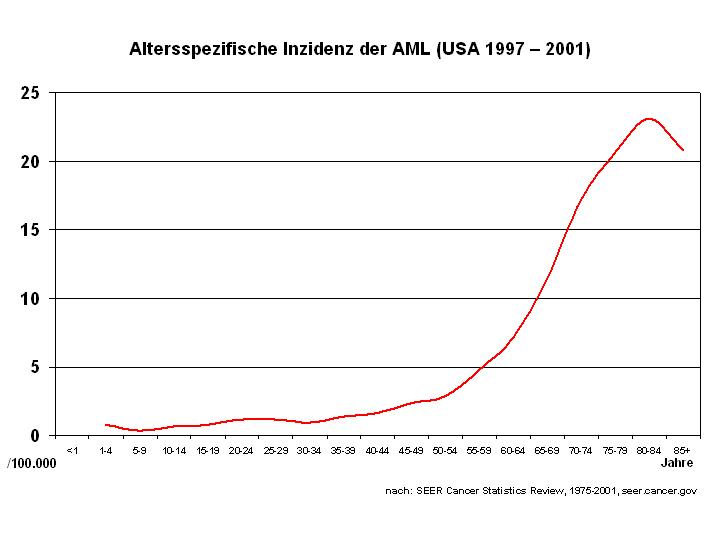
\includegraphics[width=.95\textwidth]{images/Alter_AML_2001.jpg}
\caption{Zu sehen ist die Wahrscheinlichkeit des Auftretens einer akuten myeloischen Leukämie in Abhängigkeit zum Alter. \textbf{ich suche noch nach einer aktuellen Studie}}
\label{fig:Alter_AML}
\end{figure}
Eine Leukämie kann in jeder Altersstufe auftreten, doch es gibt spezifische Altersgruppen in denen spezielle Arten der Leukämie wahrscheinlicher sind, siehe \ref{fig:Age_AML_ALL}, so treten im Kindesalter hauptsächlich akute lymphatische Leukämie (ALL) auf[Childhood acute myeloid leukaemia]. Im Erwachsenenalter hingegen ist eine AML die wahrscheinlichste Erkrankung, siehe \ref{fig:Alter_AML}.

\begin{figure}
\centering
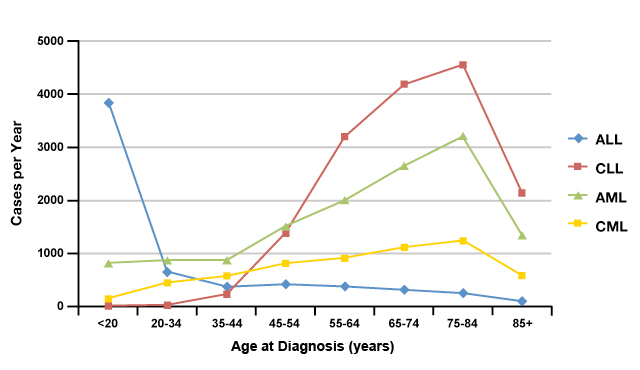
\includegraphics[width=.95\textwidth]{images/Age_AML_ALL.jpg}
\caption{Dargestellt ist die Wahrscheinlichkeit des Auftretens einer speziellen Leukämie in Abhängigkeit zum Alter. \textbf{auch hier -> aktuellen Studie kommt}}
\label{fig:Age_AML_ALL}
\end{figure}

Leukämie entsteht durch genetische Veränderungen in undifferenzierten Blutstammzellen. Wenn die Mutationen in speziellen Regionen liegen [Complex molecular genetic abnormalities in aml], so teilen sich die Zellen unkontrolliert und sind in ihrer Funktion stark eingeschränkt. Es genügt bereits eine kleine Veränderung in einer der Stammzellen, damit deren Nachkommen die gesunden Zellen verdrängen. Leider sind die Ursachen für diese genetische Modifikation im großen noch unbekannt, im allgemeinen wird jedoch vermutet, dass die spezifischen Risikofaktoren welche Krebs begünstigen auch eine Leukämie verursachen können. Durch die technische Weiterentwicklung der Länder und der damit verbundenen erhöhten Population und Lebensspanne der Menschen, steigt die Anzahl der Krebserkrankungen. Hierbei spielen Alter, Rauchen, Übergewicht, sportliche Aktivität und Reproduktionsverhalten geprägt durch die Urbanisierung eine zentrale Rolle [Global cancer statistics]. Des Weiteren ist die Aussetzung spezieller Strahlung, z.B. ionisierende Strahlung oder passive Radon Strahlung, sowie mutagene Chemikalien, diverse Viren und genetische Vorbelastung im Verdacht krebserregend zu sein.

\textbf{Behandlung? (Paper wäre gut)}
Therapie mit Zytostatika und allogene Knochenmark- bzw. Stammzelltransplantation

wie viele Menschen gehen in Remission 

Rückfallquote


%Das Ziel ist jede Mutation zuverlässig klassifizieren zu können.
%AML ist die Häufigste Erkrankung im Erwachsenen Alter
\section{Zielsetzung}

Im Universitätsklinikum Marburg in der AG Brendel wird mit dem Illumina TruSight Panel\footnote{\url{https://www.illumina.com/products/by-type/clinical-research-products/trusight-myeloid.html}} gearbeitet, um AML spezifische Regionen zu untersuchen. Dieses Panel liefert nach dem Screening eine Tabelle mit allen Mutationen des Patienten und deren Lokalisation. Auffällig dabei ist, dass die meisten Mutationen in Form von Single Nucleotide Polymorphism (SNPs) auftreten. Obwohl alle Patienten die gleichen Symptome einer AML zeigen, sind die Meisten der detektierten SNPs Patienten spezifisch und sind somit noch unbekannt und ihre Wirkung auf das entsprechende Gen kann nicht ermittelt werden. Dies hat zur Folge, dass keine Aussage über eine eventuelle Pathogenität und weiter deren Einfluss auf den Organismus getroffen werden kann.

Ziel dieser Masterarbeit ist die Entwicklung eines Programms zur Klassifizierung von SNPs aus dem \emph{Illumina TruSight Myeloid Sequencing Panel} mit Hilfe von Aminosäurerest-Pseudopotentialen.

Klassifikationen von SNPs sind eminent wichtig um ein Verständnis für die Ursachen von AML zu erhalten, doch leider haben wir in den Meisten Fällen keinerlei Informationen über die Pathogenität der gefundenen SNPs. In einer vorherigen Arbeit wurde eine Programm zum annotieren von SNPs Namens \emph{SAPA}\footnote{\url{https://github.com/TobiasJu/SAPA}} geschrieben, jedoch liefert dieses nur einen Matthews Correlation Coefficient (MCC) von 0,66 und ist damit verbesserungswürdig. 

Nun soll der Versuch unternommen werden eine Annotation der SNPs unter Zuhilfenahme der 3d Struktur zu ermöglichen. Mittels des Modells der Aminosäurerest-Pseudopotentialen soll überprüft werden, inwiefern sich Energieprofile als Datengrundlage für eine SNP Annotation in diesem Forschungsbereich eignen. Zusätzlich soll mithilfe der PDB und Pfam diejenigen Proteinfamilien ermittelt werden, welche eine aufgeklärte Struktur in der PDB besitzen, umso durch SNPs auftretende Veränderungen der PSI \& PHI Winkel, erklären zu können. Letztendlich soll getestet werden in welcher Proteindomäne der SNP liegt, z.B. in einem hoch konservierten Bereich in einer Pfam Familie liegt, um auch hiermit eine Klassifikation vorzunehmen zu können.



\section{Aufbau der Arbeit}

Zu Beginn dieser Arbeit werden die Grundlagen vermittelt, welche für die Arbeit essentiell sind. Dies beinhaltet die Erläuterung der Theorie der Aminosäurerest-Pseudopotentiale und deren Mathematischer Hintergrund. Zudem beinhaltet ein Kapitel die Erklärung der Datenbanken \emph{PDB} und \emph{Pfam}, welche als die Grundlage der PSI \& PHI Winkel Berechnung genutzt wurden. Außerdem werden auch die Grundlagen des \emph{MCCs}, \emph{Ramachandran Plots} und \emph{Homologie Moddeling} 
%und \emph{Machine Learning}
erklärt. Abschließend wird die lokale Berechnung der Energieprofile mittels Nextflow auf dem Clusters der Bioinformatics and Systems Biology Group der Justus-Liebig-Universität Gießen, kurz vorgestellt.

Nach der Vermittlung der Grundlagen, folgt ein kurzes Kapitel zu den bisherigen Erkenntnissen aus der vorangegangenen Arbeit SAPA, als Einleitung zum Hauptteil.

Der Hauptteil der Arbeit beginnt mit der Konstruktion eines adäquaten Dantesatzes, anhand vorangegangener Arbeiten. Dabei wird vor allem auf die Selektion der Daten eingegangen und deren Nutzbarkeit auf das vorliegende Problem. Anschließend wird die Erarbeitung des Programms zur Annotation der SNPs vorgestellt.

\textbf{hier fehlen noch ein Paar Schritte}

Abschließend erfolgt die Evaluation Anhand eines ClinVar Datensatzes, welcher benigne und pathogene SNPs enthält, welche von \emph{mehreren Autoren} submittiert wurden und die \emph{gleiche Annotation} beinhalten. Nach der Evaluation werden deren Ergebnisse und die Erkenntnisse der Arbeit nochmals zusammengefasst und die Aussagekraft der Klassifikation des erstellen Programms diskutiert.



%Das geht dann so \cite{Lamport95}.